\section{Blague FreeCell (Windows 7)}

\renewcommand{\CURPATH}{examples/freecell}

Ceci est une blague que j'ai fait une fois pour mes collègues qui jouaient trop
au solitaire FreeCell.
Pouvons-nous forcer FreeCell à jouer la même partie à chaque fois?
Comme, voyez-vous, dans le film ``Groundhog Day'' ?

(J'écris ceci en novembre 2019. Il semble qu'IDA ne puisse obtenir les PDBs depuis les serveurs
de Microsoft. Peut-être que Windows 7 n'est plus supporté? En tout cas, je ne peux
pas obtenir les noms de fonction...)

\subsection{Partie I}

\myindex{\CStandardLibrary!rand()}
\myindex{\CStandardLibrary!srand()}
\myindex{\CStandardLibrary!time()}
Donc, j'ai chargé FreeCell.exe dans IDA et trouvé qu'à la fois rand(), srand() et
time() sont importées depuis msvcrt.dll.
time() est en effet utilisée comme valeur d'initialisation pour srand():

\begin{lstlisting}[style=customasmx86]
.text:01029612                sub_1029612     proc near               ; CODE XREF: sub\_102615C+149
.text:01029612                                                        ; sub\_1029DA6+67
.text:01029612 8B FF                          mov     edi, edi
.text:01029614 56                             push    esi
.text:01029615 57                             push    edi
.text:01029616 6A 00                          push    0               ; Time
.text:01029618 8B F9                          mov     edi, ecx
.text:0102961A FF 15 80 16 00+                call    ds:time
.text:01029620 50                             push    eax             ; Seed
.text:01029621 FF 15 84 16 00+                call    ds:srand
.text:01029627 8B 35 AC 16 00+                mov     esi, ds:rand
.text:0102962D 59                             pop     ecx
.text:0102962E 59                             pop     ecx
.text:0102962F FF D6                          call    esi ; rand
.text:01029631 FF D6                          call    esi ; rand
.text:01029633
.text:01029633                loc_1029633:                            ; CODE XREF: sub\_1029612+26
.text:01029633                                                        ; sub\_1029612+2D
.text:01029633 FF D6                          call    esi ; rand
.text:01029635 83 F8 01                       cmp     eax, 1
.text:01029638 7C F9                          jl      short loc_1029633
.text:0102963A 3D 40 42 0F 00                 cmp     eax, 1000000
.text:0102963F 7F F2                          jg      short loc_1029633
.text:01029641 6A 01                          push    1
.text:01029643 50                             push    eax
.text:01029644 8B CF                          mov     ecx, edi
.text:01029646 E8 2D F8 FF FF                 call    sub_1028E78
.text:0102964B 5F                             pop     edi
.text:0102964C 5E                             pop     esi
.text:0102964D C3                             retn
.text:0102964D                sub_1029612     endp
\end{lstlisting}


``In the morning you will send for a hansom, desiring your man to take neither the first nor the second which may present itself.''
( The Memoirs of Sherlock Holmes, par Arthur Conan Doyle\footnote{\url{http://www.gutenberg.org/files/834/834-0.txt}} )

Il y a un autre appel a la parie time() et srand(), mais mon \tracer a montré
que ceci est notre point d'intérêt:

\begin{lstlisting}
tracer.exe -l:FreeCell.exe bpf=msvcrt.dll!time bpf=msvcrt.dll!srand,args:1

...

TID=5340|(0) msvcrt.dll!time() (called from FreeCell.exe!BASE+0x29620 (0x209620))
TID=5340|(0) msvcrt.dll!time() -> 0x5ddb68aa
TID=5340|(1) msvcrt.dll!srand(0x5ddb68aa) (called from FreeCell.exe!BASE+0x29627 (0x209627))
TID=5340|(1) msvcrt.dll!srand() -> 0x5507e0
TID=5340|(1) msvcrt.dll!srand(0x399f) (called from FreeCell.exe!BASE+0x27d3a (0x207d3a))
TID=5340|(1) msvcrt.dll!srand() -> 0x5507e0
\end{lstlisting}

Vous voyez, la fonction time() a renvoyé 0x5ddb68aa et la même valeur est utilisée
comme un argument pour srand().

Essayons de forcer time() a toujours renvoyé 0:

\begin{lstlisting}
tracer.exe -l:FreeCell.exe bpf=msvcrt.dll!time,rt:0 bpf=msvcrt.dll!srand,args:1

...

TID=2104|(0) msvcrt.dll!time() (called from FreeCell.exe!BASE+0x29620 (0xb19620))
TID=2104|(0) msvcrt.dll!time() -> 0x5ddb68f6
TID=2104|(0) Modifying EAX register to 0x0
TID=2104|(1) msvcrt.dll!srand(0x0) (called from FreeCell.exe!BASE+0x29627 (0xb19627))
TID=2104|(1) msvcrt.dll!srand() -> 0x3707e0
TID=2104|(1) msvcrt.dll!srand(0x52f6) (called from FreeCell.exe!BASE+0x27d3a (0xb17d3a))
TID=2104|(1) msvcrt.dll!srand() -> 0x3707e0
\end{lstlisting}

Maintenant, je vois toujours le même jeu à chaque fois que je lance FreeCell en
utilisant \tracer:

\begin{figure}[H]
\centering
\frame{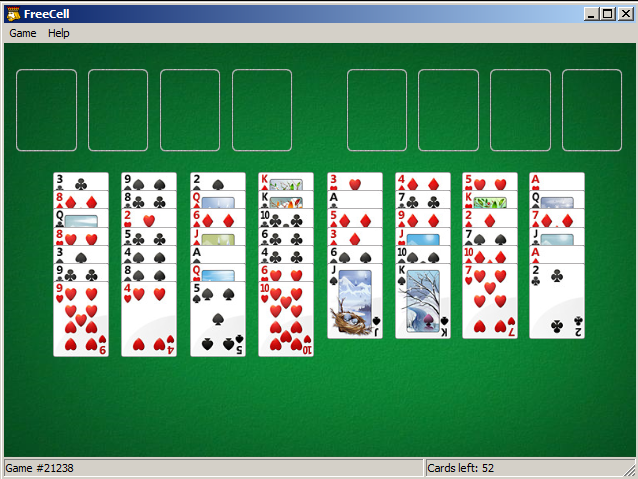
\includegraphics[width=1.0\textwidth]{\CURPATH/freecell1.png}}
\end{figure}

Maintenant, comment modifier l'exécutable?

Nous voulons passer 0 comme argument à srand() en 0x01029620.
Mais il y a une instruction sur un octet: \INS{PUSH EAX}.
Or \INS{PUSH 0} est une instruction sur deux octets. Comment la faire tenir?

Qui a-t-il dans les autres registres à ce moment? En utilisant  \tracer je les
affiche tout:

\begin{lstlisting}
tracer.exe -l:FreeCell.exe bpx=FreeCell.exe!0x01029620

...

TID=4448|(0) FreeCell.exe!0x1029620
EAX=0x5ddb6ac4 EBX=0x00000000 ECX=0x00000000 EDX=0x00000000
ESI=0x054732d0 EDI=0x054732d0 EBP=0x0020f2bc ESP=0x0020f298
EIP=0x00899620
FLAGS=PF ZF IF
TID=4448|(0) FreeCell.exe!0x1029620
EAX=0x5ddb6ac8 EBX=0x00000002 ECX=0x00000000 EDX=0x00000000
ESI=0xffffff11 EDI=0x054732d0 EBP=0x0020da78 ESP=0x0020d9d4
EIP=0x00899620
FLAGS=PF ZF IF
TID=4448|(0) FreeCell.exe!0x1029620
EAX=0x5ddb6aca EBX=0x00000002 ECX=0x00000000 EDX=0x00000000
ESI=0x7740c460 EDI=0x054732d0 EBP=0x0020da78 ESP=0x0020d9d4
EIP=0x00899620
FLAGS=PF ZF IF
...
\end{lstlisting}

Peu importe le nombre de fois que je redémaare le jeu, ECX et EDX semblent toujours
contenir 0.
Donc, j'ai modifié \INS{PUSH EAX} à l'adress 0x01029620 en \INS{PUSH EDX} (aussi
une instruction sur 1 octet), et maintenant FreeCell montre toujours le même jeu
au joueur.

Toutefois, d'autres options pourraient exister.
En fait, nous n'avons pas besoin de passer 0 à srand().
Plutôt, nous voulons passer une \emph{constante} à srand() pour que le jeu soit le
même à chaque fois.
Comme on peut le voir, la valeur d'EDI n'a pas changé. Peut-être que nous pourrions
l'essayer aussi.

Maintenant une modification un peu plus difficile.
Ouvrons FreeCell.exe dans Hiew:

\begin{figure}[H]
\centering
\frame{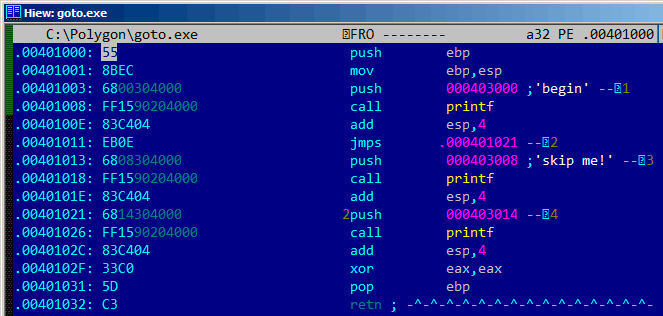
\includegraphics[width=1.0\textwidth]{\CURPATH/hiew1.png}}
\end{figure}

Nous n'avons pas des place pour remplacer l'instruction d'un octet \INS{PUSH EAX}
avec celle sur deux octets \INS{PUSH 0}.
\myindex{FIXUP}
Et nous ne pouvons pas juste remplir \verb|CALL ds:time| avec des \ac{NOP}s, car
il y a un FIXUP (adresse de la fonction time() dans msvcrt.dll).
(Hiew a marqué ces 4 octets en gris.)
Donc, voici ce que je fais: modifier les 2 premiers octets en EB 04. Ceci est un
\INS{JMP} pour contourner les 4 octets FIXUP.

\begin{figure}[H]
\centering
\frame{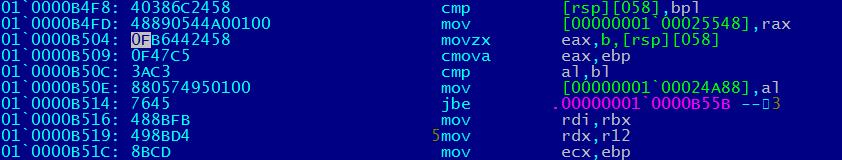
\includegraphics[width=1.0\textwidth]{\CURPATH/hiew2.png}}
\end{figure}

Puis, je remplace \INS{PUSH EAX} avec \ac{NOP}. Ainsi, srand() aura son argument du \INS{PUSH 0} au-dessus.
Aussi, je modifie une des \INS{POP ECX} en \ac{NOP}, car j'ai supprimé un \INS{PUSH}.

\begin{figure}[H]
\centering
\frame{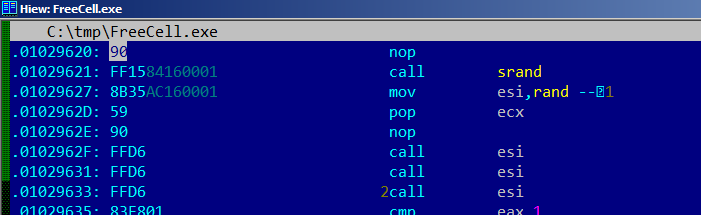
\includegraphics[width=1.0\textwidth]{\CURPATH/hiew3.png}}
\end{figure}

Maintenant, le chargeur de Windows écrita le FIXUP de 4 octets en 0x0102961C, mais
ça m'est égal: l'adresse de time() ne sera plus utilisée.

\subsection{Partie II: casser le sous-menu \emph{Select Game}}

L'utilisateur peut toujorus choisir des jeux différents dans le menu.
Voyons si srand() est toujours appelée.
J'essaye d'entrer 1/2/3 dans la boite de dialoue "Select Game":

\begin{lstlisting}
tracer.exe -l:FreeCell.exe bpf=msvcrt.dll!srand,args:1

...

TID=4936|(0) msvcrt.dll!srand(0x5ddb6df9) (called from FreeCell.exe!BASE+0x29627 (0xb49627))
TID=4936|(0) msvcrt.dll!srand() -> 0x5907e0
TID=4936|(0) msvcrt.dll!srand(0x2b40) (called from FreeCell.exe!BASE+0x27d3a (0xb47d3a))
TID=4936|(0) msvcrt.dll!srand() -> 0x5907e0
TID=4936|(0) msvcrt.dll!srand(0x1) (called from FreeCell.exe!BASE+0x27d3a (0xb47d3a))
TID=4936|(0) msvcrt.dll!srand() -> 0x5907e0
TID=4936|(0) msvcrt.dll!srand(0x2) (called from FreeCell.exe!BASE+0x27d3a (0xb47d3a))
TID=4936|(0) msvcrt.dll!srand() -> 0x5907e0
TID=4936|(0) msvcrt.dll!srand(0x3) (called from FreeCell.exe!BASE+0x27d3a (0xb47d3a))
TID=4936|(0) msvcrt.dll!srand() -> 0x5907e0
\end{lstlisting}

Oui, le nombre qu'entre l'utilisateur est simplement un argument pour srand().
Où est-elle appelée?

\begin{lstlisting}
.text:01027CBA                loc_1027CBA:                            ; CODE XREF: sub\_1027AC6+179
.text:01027CBA 83 FF FC                       cmp     edi, 0FFFFFFFCh
.text:01027CBD 75 74                          jnz     short loc_1027D33

...

.text:01027D33                loc_1027D33:                            ; CODE XREF: sub\_1027AC6+1F7
.text:01027D33 57                             push    edi             ; Seed
.text:01027D34 FF 15 84 16 00+                call    ds:srand
.text:01027D3A 59                             pop     ecx
.text:01027D3B 6A 34                          push    34h
.text:01027D3D 5B                             pop     ebx
.text:01027D3E 33 C0                          xor     eax, eax
\end{lstlisting}

Je n'ai pas pu modifier \INS{PUSH EDI} d'un octet en \INS{PUSH 0} de deux octets.
Mais je vois qu'il y seulement un unique saut à \verb|loc_1027D33| dans ce qui précède.

Je modifie \INS{CMP EDI, ...} en \INS{XOR EDI, EDI}, en complètant le 3ème octet
avec \ac{NOP}.
Je modifie aussi JNZ en JMP, afin que le saut se produise toujours.

Maintenant FreeCell ignore le nombre entré par l'utilisateur, mais soudain, il y
a le même jeu au début:

\begin{figure}[H]
\centering
\frame{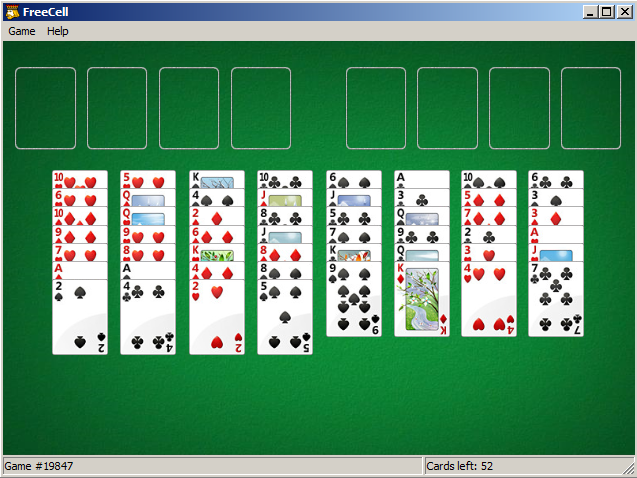
\includegraphics[width=1.0\textwidth]{\CURPATH/freecell2.png}}
\end{figure}

Il semble que le code que nous avons modifié dans la partie I est relié d'une certaine
façon à du code après 0x01027CBD, qui s'exécute si EDI==0xFFFFFFFC.
De toutes façons, notre but est atteint --- le jeu est toujours le même au début,
et l'utilisateur ne peut pas en choisir un autre avec le menu.
